\documentclass[a4paper, body={18cm,22cm}]{article}
\usepackage{ctex}
\usepackage{amsmath}
\usepackage{tikz}
\usepackage{xparse}
\usetikzlibrary{automata, positioning}


\title{Homework2: NFA-DFA}
\author{李鹏达 10225101460}
\date{}

\RenewDocumentCommand{\t}{m m O{\varepsilon} O{auto}}{%
\path[->] (#1) edge [#4]node {$#3$} (#2);
}

\begin{document}

\maketitle
\subsection*{一、使用 Thompson 构造法为下列正规式构造 NFA,写出每个 NFA 处理符号串 ``ababbab'' 过程中的状态转换序列。}

\begin{enumerate}
    \item[a)] \((a|b)^*\)
    
    \begin{center}
        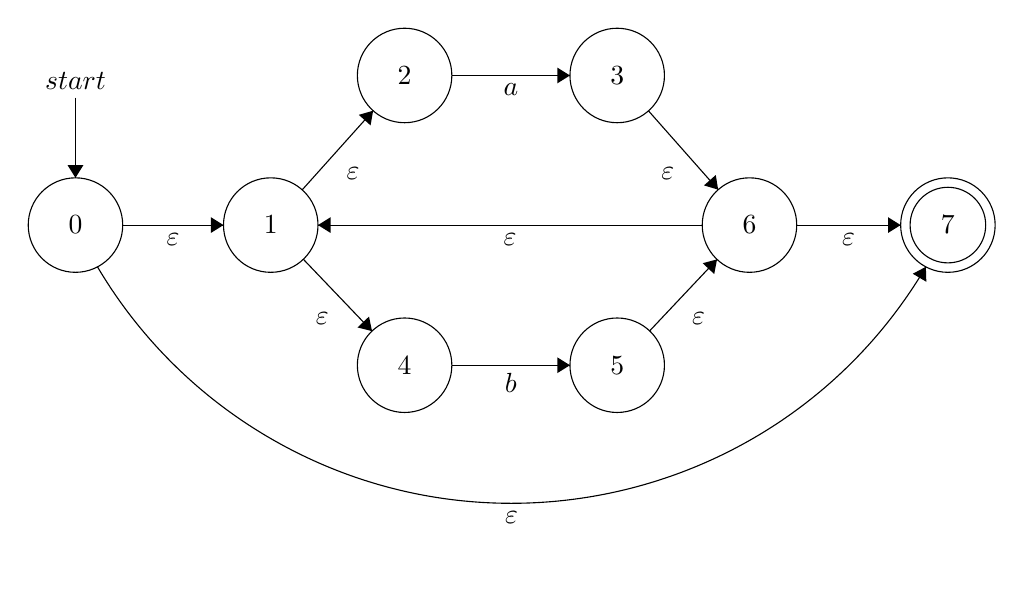
\begin{tikzpicture}[scale=0.2]
        \tikzstyle{every node}+=[inner sep=0pt]
        \draw [black] (3.7,-32.8) circle (3);
        \draw (3.7,-32.8) node {$0$};
        \draw [black] (16.1,-32.8) circle (3);
        \draw (16.1,-32.8) node {$1$};
        \draw [black] (24.6,-23.3) circle (3);
        \draw (24.6,-23.3) node {$2$};
        \draw [black] (38.1,-23.3) circle (3);
        \draw (38.1,-23.3) node {$3$};
        \draw [black] (24.6,-41.7) circle (3);
        \draw (24.6,-41.7) node {$4$};
        \draw [black] (38.1,-41.7) circle (3);
        \draw (38.1,-41.7) node {$5$};
        \draw [black] (46.5,-32.8) circle (3);
        \draw (46.5,-32.8) node {$6$};
        \draw [black] (59.1,-32.8) circle (3);
        \draw (59.1,-32.8) node {$7$};
        \draw [black] (59.1,-32.8) circle (2.4);
        \draw [black] (6.7,-32.8) -- (13.1,-32.8);
        \fill [black] (13.1,-32.8) -- (12.3,-32.3) -- (12.3,-33.3);
        \draw (9.9,-33.3) node [below] {$\varepsilon$};
        \draw [black] (18.1,-30.56) -- (22.6,-25.54);
        \fill [black] (22.6,-25.54) -- (21.69,-25.8) -- (22.44,-26.47);
        \draw (20.89,-29.51) node [right] {$\varepsilon$};
        \draw [black] (27.6,-23.3) -- (35.1,-23.3);
        \fill [black] (35.1,-23.3) -- (34.3,-22.8) -- (34.3,-23.8);
        \draw (31.35,-23.8) node [below] {$a$};
        \draw [black] (18.17,-34.97) -- (22.53,-39.53);
        \fill [black] (22.53,-39.53) -- (22.34,-38.61) -- (21.61,-39.3);
        \draw (19.82,-38.72) node [left] {$\varepsilon$};
        \draw [black] (27.6,-41.7) -- (35.1,-41.7);
        \fill [black] (35.1,-41.7) -- (34.3,-41.2) -- (34.3,-42.2);
        \draw (31.35,-42.2) node [below] {$b$};
        \draw [black] (40.16,-39.52) -- (44.44,-34.98);
        \fill [black] (44.44,-34.98) -- (43.53,-35.22) -- (44.26,-35.91);
        \draw (42.83,-38.72) node [right] {$\varepsilon$};
        \draw [black] (40.09,-25.55) -- (44.51,-30.55);
        \fill [black] (44.51,-30.55) -- (44.36,-29.62) -- (43.61,-30.28);
        \draw (41.76,-29.5) node [left] {$\varepsilon$};
        \draw [black] (3.7,-24.7) -- (3.7,-29.8);
        \draw (3.7,-24.2) node [above] {$start$};
        \fill [black] (3.7,-29.8) -- (4.2,-29) -- (3.2,-29);
        \draw [black] (43.5,-32.8) -- (19.1,-32.8);
        \fill [black] (19.1,-32.8) -- (19.9,-33.3) -- (19.9,-32.3);
        \draw (31.3,-33.3) node [below] {$\varepsilon$};
        \draw [black] (49.5,-32.8) -- (56.1,-32.8);
        \fill [black] (56.1,-32.8) -- (55.3,-32.3) -- (55.3,-33.3);
        \draw (52.8,-33.3) node [below] {$\varepsilon$};
        \draw [black] (57.703,-35.454) arc (-30.57848:-149.42152:30.552);
        \fill [black] (57.7,-35.45) -- (56.87,-35.89) -- (57.73,-36.4);
        \draw (31.4,-50.96) node [below] {$\varepsilon$};
        \end{tikzpicture}
        \end{center}

    $ababbab$

    $0 \to 1 \to 2 \to 3 \to 6 \to 1 \to 4 \to 5 \to 6 \\
    \to 1 \to 2 \to 3 \to 6 \to 1 \to 4 \to 5 \to 6 \\
    \to 1 \to 4 \to 5 \to 6 \to 1 \to 2 \to 3 \to 6 \\
    \to 1 \to 4 \to 5 \to 6 \to 7
    $

    \newpage
    \item[b)] \((a^*|b^*)^*\)
    
    \begin{center}
        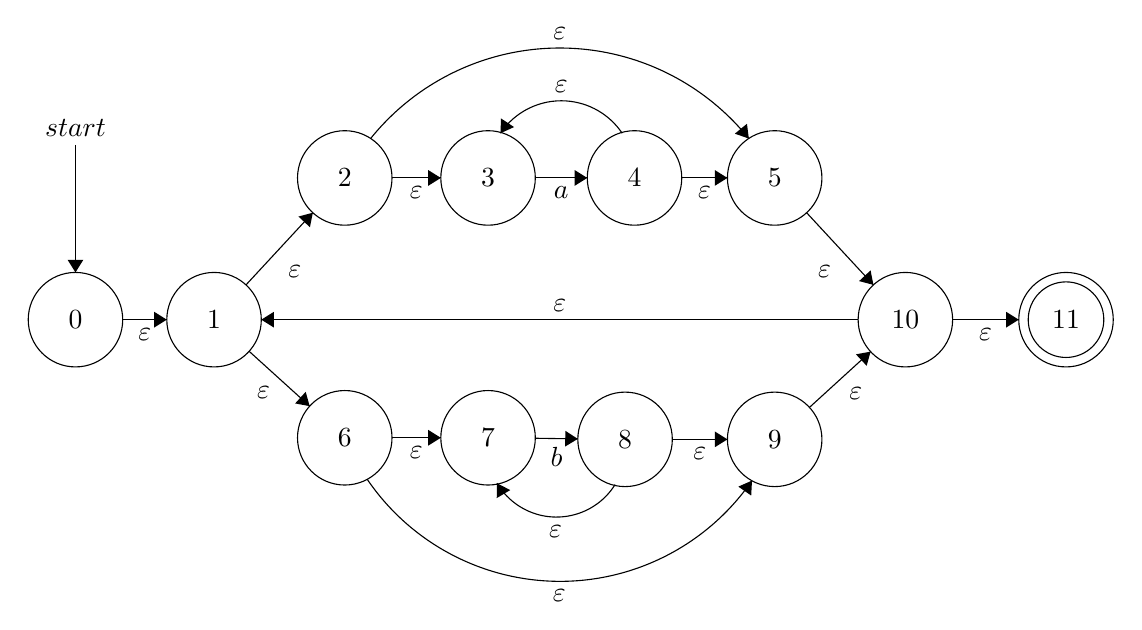
\begin{tikzpicture}[scale=0.2]
        \tikzstyle{every node}+=[inner sep=0pt]
        \draw [black] (5,-29.8) circle (3);
        \draw (5,-29.8) node {$0$};
        \draw [black] (13.8,-29.8) circle (3);
        \draw (13.8,-29.8) node {$1$};
        \draw [black] (22.1,-20.8) circle (3);
        \draw (22.1,-20.8) node {$2$};
        \draw [black] (31.2,-20.8) circle (3);
        \draw (31.2,-20.8) node {$3$};
        \draw [black] (40.5,-20.8) circle (3);
        \draw (40.5,-20.8) node {$4$};
        \draw [black] (49.4,-20.8) circle (3);
        \draw (49.4,-20.8) node {$5$};
        \draw [black] (22.1,-37.3) circle (3);
        \draw (22.1,-37.3) node {$6$};
        \draw [black] (31.2,-37.3) circle (3);
        \draw (31.2,-37.3) node {$7$};
        \draw [black] (39.9,-37.4) circle (3);
        \draw (39.9,-37.4) node {$8$};
        \draw [black] (49.4,-37.4) circle (3);
        \draw (49.4,-37.4) node {$9$};
        \draw [black] (57.7,-29.8) circle (3);
        \draw (57.7,-29.8) node {$10$};
        \draw [black] (67.9,-29.8) circle (3);
        \draw (67.9,-29.8) node {$11$};
        \draw [black] (67.9,-29.8) circle (2.4);
        \draw [black] (8,-29.8) -- (10.8,-29.8);
        \fill [black] (10.8,-29.8) -- (10,-29.3) -- (10,-30.3);
        \draw (9.4,-30.3) node [below] {$\varepsilon$};
        \draw [black] (15.83,-27.59) -- (20.07,-23.01);
        \fill [black] (20.07,-23.01) -- (19.16,-23.25) -- (19.89,-23.93);
        \draw (18.48,-26.76) node [right] {$\varepsilon$};
        \draw [black] (25.1,-20.8) -- (28.2,-20.8);
        \fill [black] (28.2,-20.8) -- (27.4,-20.3) -- (27.4,-21.3);
        \draw (26.65,-21.3) node [below] {$\varepsilon$};
        \draw [black] (34.2,-20.8) -- (37.5,-20.8);
        \fill [black] (37.5,-20.8) -- (36.7,-20.3) -- (36.7,-21.3);
        \draw (35.85,-21.3) node [below] {$a$};
        \draw [black] (43.5,-20.8) -- (46.4,-20.8);
        \fill [black] (46.4,-20.8) -- (45.6,-20.3) -- (45.6,-21.3);
        \draw (44.95,-21.3) node [below] {$\varepsilon$};
        \draw [black] (34.2,-37.33) -- (36.9,-37.37);
        \fill [black] (36.9,-37.37) -- (36.11,-36.86) -- (36.09,-37.86);
        \draw (35.55,-37.86) node [below] {$b$};
        \draw [black] (16.03,-31.81) -- (19.87,-35.29);
        \fill [black] (19.87,-35.29) -- (19.62,-34.38) -- (18.95,-35.12);
        \draw (16.94,-34.04) node [below] {$\varepsilon$};
        \draw [black] (25.1,-37.3) -- (28.2,-37.3);
        \fill [black] (28.2,-37.3) -- (27.4,-36.8) -- (27.4,-37.8);
        \draw (26.65,-37.8) node [below] {$\varepsilon$};
        \draw [black] (42.9,-37.4) -- (46.4,-37.4);
        \fill [black] (46.4,-37.4) -- (45.6,-36.9) -- (45.6,-37.9);
        \draw (44.65,-37.9) node [below] {$\varepsilon$};
        \draw [black] (51.61,-35.37) -- (55.49,-31.83);
        \fill [black] (55.49,-31.83) -- (54.56,-32) -- (55.24,-32.73);
        \draw (54.56,-34.09) node [below] {$\varepsilon$};
        \draw [black] (60.7,-29.8) -- (64.9,-29.8);
        \fill [black] (64.9,-29.8) -- (64.1,-29.3) -- (64.1,-30.3);
        \draw (62.8,-30.3) node [below] {$\varepsilon$};
        \draw [black] (51.43,-23.01) -- (55.67,-27.59);
        \fill [black] (55.67,-27.59) -- (55.49,-26.67) -- (54.76,-27.35);
        \draw (53.02,-26.76) node [left] {$\varepsilon$};
        \draw [black] (5,-18.7) -- (5,-26.8);
        \draw (5,-18.2) node [above] {$start$};
        \fill [black] (5,-26.8) -- (5.5,-26) -- (4.5,-26);
        \draw [black] (31.986,-17.958) arc (-213.91159:-326.08841:4.656);
        \fill [black] (31.99,-17.96) -- (32.85,-17.57) -- (32.02,-17.02);
        \draw (35.85,-15.4) node [above] {$\varepsilon$};
        \draw [black] (39.265,-40.273) arc (-32.04278:-149.2743:4.391);
        \fill [black] (31.77,-40.19) -- (31.75,-41.13) -- (32.61,-40.62);
        \draw (35.49,-42.84) node [below] {$\varepsilon$};
        \draw [black] (23.743,-18.296) arc (141.15127:38.84873:15.417);
        \fill [black] (47.76,-18.3) -- (47.64,-17.36) -- (46.87,-17.99);
        \draw (35.75,-12.05) node [above] {$\varepsilon$};
        \draw [black] (47.956,-40.024) arc (-34.63142:-145.78833:14.809);
        \fill [black] (47.96,-40.02) -- (47.09,-40.4) -- (47.91,-40.97);
        \draw (35.72,-46.92) node [below] {$\varepsilon$};
        \draw [black] (54.7,-29.8) -- (16.8,-29.8);
        \fill [black] (16.8,-29.8) -- (17.6,-30.3) -- (17.6,-29.3);
        \draw (35.75,-29.3) node [above] {$\varepsilon$};
        \end{tikzpicture}
        \end{center}

    $ababbab$

    $0 \to 1 \to 2 \to 3 \to 4 \to 5 \to 10 \\
     \to 1 \to 6 \to 7 \to 8 \to 9 \to 10 \\
        \to 1 \to 2 \to 3 \to 4 \to 5 \to 10 \\
        \to 1 \to 6 \to 7 \to 8 \to 7 \to 8 \to 9 \to 10 \\
        \to 1 \to 2 \to 3 \to 4 \to 5 \to 10 \\
        \to 1 \to 6 \to 7 \to 8 \to 9 \to 10 \to 11 
    $

    \newpage
    \item[c)] \(((\varepsilon|a)b^*)^*\)
    
    \begin{center}
        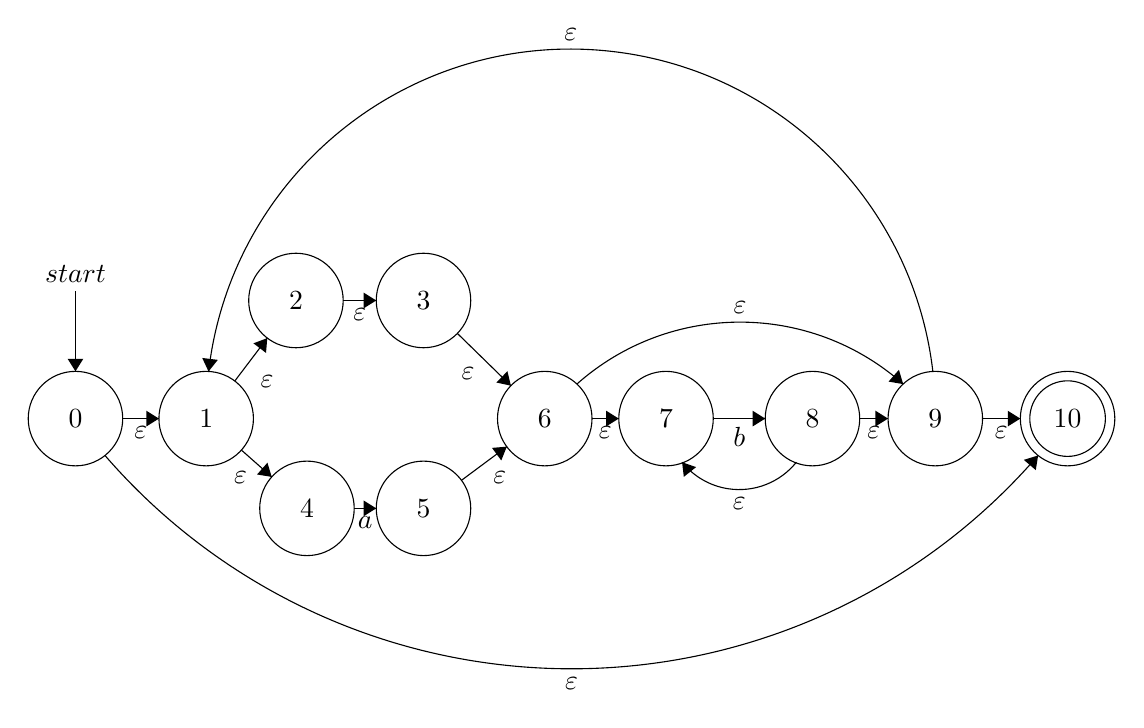
\begin{tikzpicture}[scale=0.2]
        \tikzstyle{every node}+=[inner sep=0pt]
        \draw [black] (4.8,-28.4) circle (3);
        \draw (4.8,-28.4) node {$0$};
        \draw [black] (13.1,-28.4) circle (3);
        \draw (13.1,-28.4) node {$1$};
        \draw [black] (18.8,-20.9) circle (3);
        \draw (18.8,-20.9) node {$2$};
        \draw [black] (26.9,-20.9) circle (3);
        \draw (26.9,-20.9) node {$3$};
        \draw [black] (19.5,-34.1) circle (3);
        \draw (19.5,-34.1) node {$4$};
        \draw [black] (26.9,-34.1) circle (3);
        \draw (26.9,-34.1) node {$5$};
        \draw [black] (34.6,-28.4) circle (3);
        \draw (34.6,-28.4) node {$6$};
        \draw [black] (42.3,-28.4) circle (3);
        \draw (42.3,-28.4) node {$7$};
        \draw [black] (51.6,-28.4) circle (3);
        \draw (51.6,-28.4) node {$8$};
        \draw [black] (59.4,-28.4) circle (3);
        \draw (59.4,-28.4) node {$9$};
        \draw [black] (67.8,-28.4) circle (3);
        \draw (67.8,-28.4) node {$10$};
        \draw [black] (67.8,-28.4) circle (2.4);
        \draw [black] (7.8,-28.4) -- (10.1,-28.4);
        \fill [black] (10.1,-28.4) -- (9.3,-27.9) -- (9.3,-28.9);
        \draw (8.95,-28.9) node [below] {$\varepsilon$};
        \draw [black] (14.92,-26.01) -- (16.98,-23.29);
        \fill [black] (16.98,-23.29) -- (16.1,-23.62) -- (16.9,-24.23);
        \draw (16.52,-26.05) node [right] {$\varepsilon$};
        \draw [black] (21.8,-20.9) -- (23.9,-20.9);
        \fill [black] (23.9,-20.9) -- (23.1,-20.4) -- (23.1,-21.4);
        \draw (22.85,-21.4) node [below] {$\varepsilon$};
        \draw [black] (15.34,-30.4) -- (17.26,-32.1);
        \fill [black] (17.26,-32.1) -- (16.99,-31.2) -- (16.33,-31.95);
        \draw (15.29,-31.74) node [below] {$\varepsilon$};
        \draw [black] (22.5,-34.1) -- (23.9,-34.1);
        \fill [black] (23.9,-34.1) -- (23.1,-33.6) -- (23.1,-34.6);
        \draw (23.2,-34.6) node [below] {$a$};
        \draw [black] (29.31,-32.32) -- (32.19,-30.18);
        \fill [black] (32.19,-30.18) -- (31.25,-30.26) -- (31.84,-31.06);
        \draw (31.75,-31.75) node [below] {$\varepsilon$};
        \draw [black] (29.05,-22.99) -- (32.45,-26.31);
        \fill [black] (32.45,-26.31) -- (32.23,-25.39) -- (31.53,-26.11);
        \draw (29.73,-25.13) node [below] {$\varepsilon$};
        \draw [black] (37.6,-28.4) -- (39.3,-28.4);
        \fill [black] (39.3,-28.4) -- (38.5,-27.9) -- (38.5,-28.9);
        \draw (38.45,-28.9) node [below] {$\varepsilon$};
        \draw [black] (45.3,-28.4) -- (48.6,-28.4);
        \fill [black] (48.6,-28.4) -- (47.8,-27.9) -- (47.8,-28.9);
        \draw (46.95,-28.9) node [below] {$b$};
        \draw [black] (54.6,-28.4) -- (56.4,-28.4);
        \fill [black] (56.4,-28.4) -- (55.6,-27.9) -- (55.6,-28.9);
        \draw (55.5,-28.9) node [below] {$\varepsilon$};
        \draw [black] (62.4,-28.4) -- (64.8,-28.4);
        \fill [black] (64.8,-28.4) -- (64,-27.9) -- (64,-28.9);
        \draw (63.6,-28.9) node [below] {$\varepsilon$};
        \draw [black] (50.579,-31.166) arc (-38.73213:-141.26787:4.652);
        \fill [black] (43.32,-31.17) -- (43.43,-32.1) -- (44.21,-31.48);
        \draw (46.95,-33.41) node [below] {$\varepsilon$};
        \draw [black] (36.64,-26.206) arc (131.58004:48.41996:15.611);
        \fill [black] (57.36,-26.21) -- (57.09,-25.3) -- (56.43,-26.05);
        \draw (47,-21.77) node [above] {$\varepsilon$};
        \draw [black] (13.254,-25.406) arc (-186.64901:-353.35099:23.152);
        \fill [black] (13.25,-25.41) -- (13.84,-24.67) -- (12.85,-24.55);
        \draw (36.25,-4.43) node [above] {$\varepsilon$};
        \draw [black] (65.926,-30.742) arc (-40.86001:-139.13999:39.172);
        \fill [black] (65.93,-30.74) -- (65.02,-31.02) -- (65.78,-31.67);
        \draw (36.3,-44.79) node [below] {$\varepsilon$};
        \draw [black] (4.8,-20.3) -- (4.8,-25.4);
        \draw (4.8,-19.8) node [above] {$start$};
        \fill [black] (4.8,-25.4) -- (5.3,-24.6) -- (4.3,-24.6);
        \end{tikzpicture}
        \end{center}

    $ababbab$

    $0 \to 1 \to 4 \to5\to6\to7\to8\to9\\
    \to 1 \to 4 \to5\to6\to7\to8\to7\to8\to9\\
    \to 1 \to 4 \to5\to6\to7\to8\to9 \to 10
    $

    \newpage
    
    \item[d)] \((a|b)^* abb (a|b)^*\)
    
    \begin{center}
        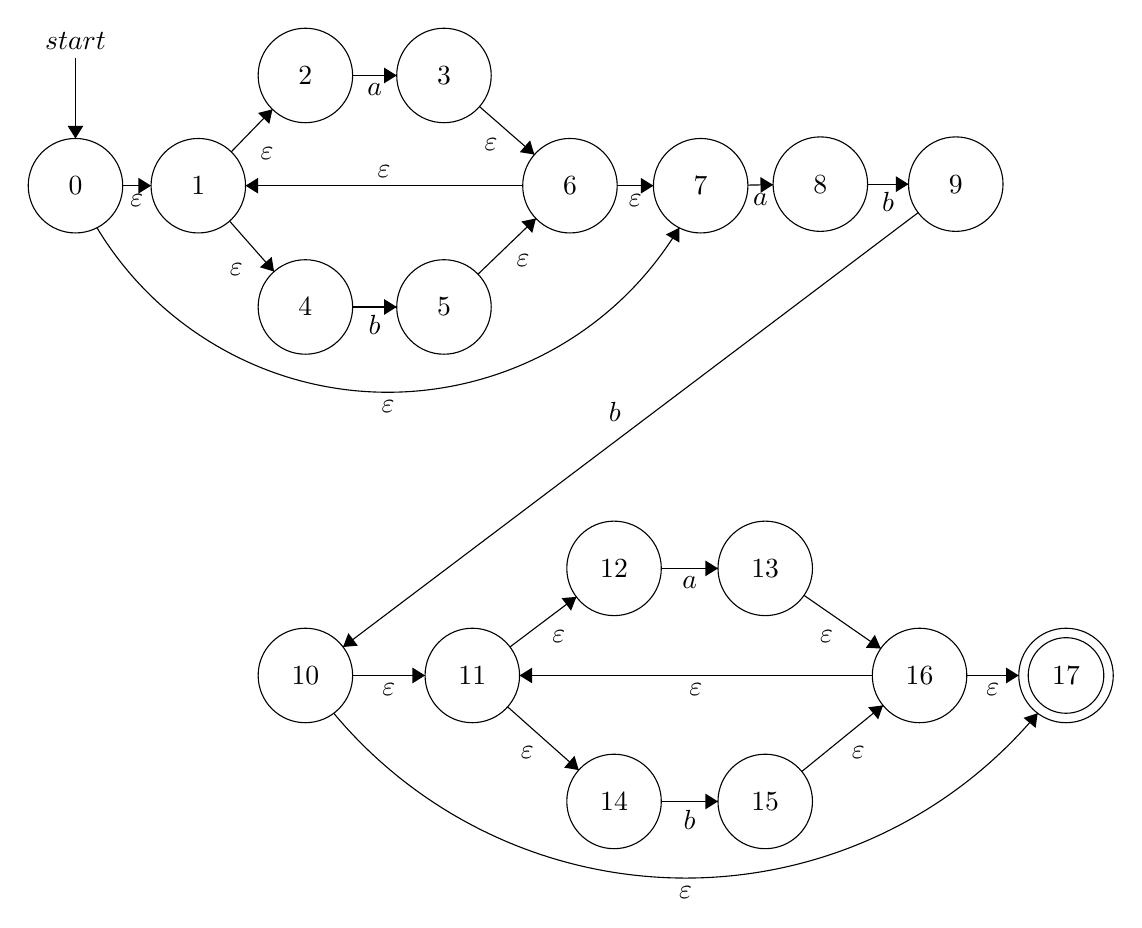
\begin{tikzpicture}[scale=0.2]
        \tikzstyle{every node}+=[inner sep=0pt]
        \draw [black] (4.1,-13.1) circle (3);
        \draw (4.1,-13.1) node {$0$};
        \draw [black] (11.9,-13.1) circle (3);
        \draw (11.9,-13.1) node {$1$};
        \draw [black] (18.7,-6.1) circle (3);
        \draw (18.7,-6.1) node {$2$};
        \draw [black] (27.5,-6.1) circle (3);
        \draw (27.5,-6.1) node {$3$};
        \draw [black] (18.7,-20.8) circle (3);
        \draw (18.7,-20.8) node {$4$};
        \draw [black] (27.5,-20.8) circle (3);
        \draw (27.5,-20.8) node {$5$};
        \draw [black] (35.5,-13.1) circle (3);
        \draw (35.5,-13.1) node {$6$};
        \draw [black] (43.8,-13.1) circle (3);
        \draw (43.8,-13.1) node {$7$};
        \draw [black] (51.4,-13) circle (3);
        \draw (51.4,-13) node {$8$};
        \draw [black] (60,-13) circle (3);
        \draw (60,-13) node {$9$};
        \draw [black] (18.7,-44.2) circle (3);
        \draw (18.7,-44.2) node {$10$};
        \draw [black] (29.3,-44.2) circle (3);
        \draw (29.3,-44.2) node {$11$};
        \draw [black] (38.3,-37.4) circle (3);
        \draw (38.3,-37.4) node {$12$};
        \draw [black] (47.9,-37.4) circle (3);
        \draw (47.9,-37.4) node {$13$};
        \draw [black] (38.3,-52.2) circle (3);
        \draw (38.3,-52.2) node {$14$};
        \draw [black] (47.9,-52.2) circle (3);
        \draw (47.9,-52.2) node {$15$};
        \draw [black] (57.7,-44.2) circle (3);
        \draw (57.7,-44.2) node {$16$};
        \draw [black] (67,-44.2) circle (3);
        \draw (67,-44.2) node {$17$};
        \draw [black] (67,-44.2) circle (2.4);
        \draw [black] (7.1,-13.1) -- (8.9,-13.1);
        \fill [black] (8.9,-13.1) -- (8.1,-12.6) -- (8.1,-13.6);
        \draw (8,-13.6) node [below] {$\varepsilon$};
        \draw [black] (13.99,-10.95) -- (16.61,-8.25);
        \fill [black] (16.61,-8.25) -- (15.69,-8.48) -- (16.41,-9.17);
        \draw (15.83,-11.07) node [right] {$\varepsilon$};
        \draw [black] (21.7,-6.1) -- (24.5,-6.1);
        \fill [black] (24.5,-6.1) -- (23.7,-5.6) -- (23.7,-6.6);
        \draw (23.1,-6.6) node [below] {$a$};
        \draw [black] (13.89,-15.35) -- (16.71,-18.55);
        \fill [black] (16.71,-18.55) -- (16.56,-17.62) -- (15.81,-18.28);
        \draw (14.76,-18.4) node [left] {$\varepsilon$};
        \draw [black] (21.7,-20.8) -- (24.5,-20.8);
        \fill [black] (24.5,-20.8) -- (23.7,-20.3) -- (23.7,-21.3);
        \draw (23.1,-21.3) node [below] {$b$};
        \draw [black] (29.66,-18.72) -- (33.34,-15.18);
        \fill [black] (33.34,-15.18) -- (32.42,-15.37) -- (33.11,-16.1);
        \draw (32.52,-17.43) node [below] {$\varepsilon$};
        \draw [black] (29.76,-8.08) -- (33.24,-11.12);
        \fill [black] (33.24,-11.12) -- (32.97,-10.22) -- (32.31,-10.97);
        \draw (30.49,-10.09) node [below] {$\varepsilon$};
        \draw [black] (4.1,-5) -- (4.1,-10.1);
        \draw (4.1,-4.5) node [above] {$start$};
        \fill [black] (4.1,-10.1) -- (4.6,-9.3) -- (3.6,-9.3);
        \draw [black] (32.5,-13.1) -- (14.9,-13.1);
        \fill [black] (14.9,-13.1) -- (15.7,-13.6) -- (15.7,-12.6);
        \draw (23.7,-12.6) node [above] {$\varepsilon$};
        \draw [black] (38.5,-13.1) -- (40.8,-13.1);
        \fill [black] (40.8,-13.1) -- (40,-12.6) -- (40,-13.6);
        \draw (39.65,-13.6) node [below] {$\varepsilon$};
        \draw [black] (42.435,-15.769) arc (-31.06689:-148.93311:21.581);
        \fill [black] (42.44,-15.77) -- (41.59,-16.2) -- (42.45,-16.71);
        \draw (23.95,-26.71) node [below] {$\varepsilon$};
        \draw [black] (46.8,-13.06) -- (48.4,-13.04);
        \fill [black] (48.4,-13.04) -- (47.59,-12.55) -- (47.61,-13.55);
        \draw (47.6,-13.56) node [below] {$a$};
        \draw [black] (54.4,-13) -- (57,-13);
        \fill [black] (57,-13) -- (56.2,-12.5) -- (56.2,-13.5);
        \draw (55.7,-13.5) node [below] {$b$};
        \draw [black] (57.61,-14.81) -- (21.09,-42.39);
        \fill [black] (21.09,-42.39) -- (22.03,-42.31) -- (21.43,-41.51);
        \draw (38.35,-28.1) node [above] {$b$};
        \draw [black] (21.7,-44.2) -- (26.3,-44.2);
        \fill [black] (26.3,-44.2) -- (25.5,-43.7) -- (25.5,-44.7);
        \draw (24,-44.7) node [below] {$\varepsilon$};
        \draw [black] (31.69,-42.39) -- (35.91,-39.21);
        \fill [black] (35.91,-39.21) -- (34.97,-39.29) -- (35.57,-40.09);
        \draw (34.8,-41.3) node [below] {$\varepsilon$};
        \draw [black] (41.3,-37.4) -- (44.9,-37.4);
        \fill [black] (44.9,-37.4) -- (44.1,-36.9) -- (44.1,-37.9);
        \draw (43.1,-37.9) node [below] {$a$};
        \draw [black] (41.3,-52.2) -- (44.9,-52.2);
        \fill [black] (44.9,-52.2) -- (44.1,-51.7) -- (44.1,-52.7);
        \draw (43.1,-52.7) node [below] {$b$};
        \draw [black] (50.36,-39.11) -- (55.24,-42.49);
        \fill [black] (55.24,-42.49) -- (54.86,-41.62) -- (54.29,-42.44);
        \draw (51.8,-41.3) node [below] {$\varepsilon$};
        \draw [black] (50.22,-50.3) -- (55.38,-46.1);
        \fill [black] (55.38,-46.1) -- (54.44,-46.22) -- (55.07,-46.99);
        \draw (53.81,-48.69) node [below] {$\varepsilon$};
        \draw [black] (31.54,-46.19) -- (36.06,-50.21);
        \fill [black] (36.06,-50.21) -- (35.79,-49.3) -- (35.13,-50.05);
        \draw (32.79,-48.69) node [below] {$\varepsilon$};
        \draw [black] (60.7,-44.2) -- (64,-44.2);
        \fill [black] (64,-44.2) -- (63.2,-43.7) -- (63.2,-44.7);
        \draw (62.35,-44.7) node [below] {$\varepsilon$};
        \draw [black] (54.7,-44.2) -- (32.3,-44.2);
        \fill [black] (32.3,-44.2) -- (33.1,-44.7) -- (33.1,-43.7);
        \draw (43.5,-44.7) node [below] {$\varepsilon$};
        \draw [black] (65.201,-46.599) arc (-39.81877:-140.18123:29.1);
        \fill [black] (65.2,-46.6) -- (64.3,-46.89) -- (65.07,-47.53);
        \draw (42.85,-57.56) node [below] {$\varepsilon$};
        \end{tikzpicture}
        \end{center}

        $ababbab$

        $0 \to 1 \to 2 \to 3 \to 6\\
         \to 1 \to 4 \to 5 \to 6 \to 7 \\
        \to 8 \to 9\\
         \to 10 \to 11 \to 12 \to 13 \to 16\\
          \to 11 \to 14 \to 15 \to 16 \to 17$
\end{enumerate}

\newpage
\subsection*{二、利用子集构造法将第一题得到的 NFA 转换为 DFA,同样写出分析符号串 ``ababbab'' 过程中的状态转换。}


\newcommand{\ec}[1]{\textrm{$\varepsilon$-closure}(\{#1\})}
\newcommand{\ecc}[1]{\textrm{$\varepsilon$-closure}(#1)}
\newcommand{\mv}[2]{\textrm{move}(#1,#2)}
\begin{enumerate}
    \item[a)] \((a|b)^*\)
    
    $\ec{0} = \{0, 1, 2, 4, 7\} = S_0\\
    \ecc{\mv{S_0}{a}} = \ec{3} = \{1,2,3,4,6,7\} = S_1\\
    \ecc{\mv{s_0}{b}} = \ec{5} = \{1,2,4,5,6,7\} = S_2\\
    \ecc{\mv{S_1}{a}} = \ec{3} = S_1\\
    \ecc{\mv{S_1}{b}} = \ec{5} = S_2\\
    \ecc{\mv{S_2}{a}} = \ec{3} = S_1\\
    \ecc{\mv{S_2}{b}} = \ec{5} = S_2\\
    $

    \begin{center}
        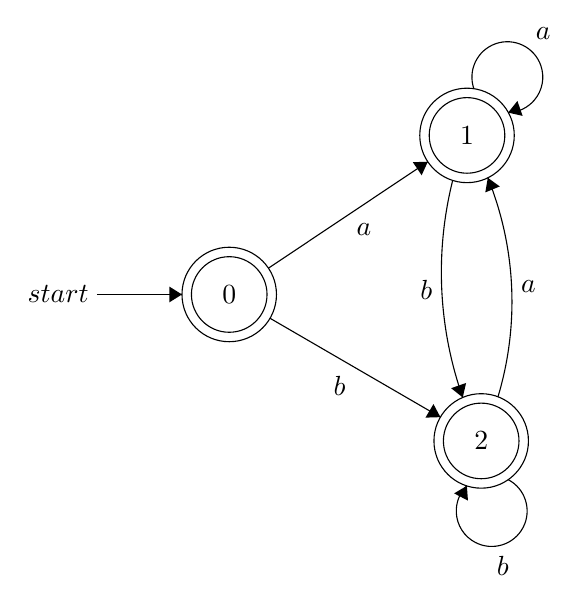
\begin{tikzpicture}[scale=0.2]
        \tikzstyle{every node}+=[inner sep=0pt]
        \draw [black] (16.6,-28.8) circle (3);
        \draw (16.6,-28.8) node {$0$};
        \draw [black] (16.6,-28.8) circle (2.4);
        \draw [black] (31.7,-18.7) circle (3);
        \draw (31.7,-18.7) node {$1$};
        \draw [black] (31.7,-18.7) circle (2.4);
        \draw [black] (32.6,-38.1) circle (3);
        \draw (32.6,-38.1) node {$2$};
        \draw [black] (32.6,-38.1) circle (2.4);
        \draw [black] (19.09,-27.13) -- (29.21,-20.37);
        \fill [black] (29.21,-20.37) -- (28.26,-20.4) -- (28.82,-21.23);
        \draw (25.15,-24.25) node [below] {$a$};
        \draw [black] (19.19,-30.31) -- (30.01,-36.59);
        \fill [black] (30.01,-36.59) -- (29.57,-35.76) -- (29.06,-36.62);
        \draw (23.6,-33.95) node [below] {$b$};
        \draw [black] (32.138,-15.744) arc (199.30485:-88.69515:2.25);
        \draw (36.54,-12.65) node [above] {$a$};
        \fill [black] (34.31,-17.25) -- (35.23,-17.46) -- (34.9,-16.51);
        \draw [black] (31.43,-35.34) arc (-160.61096:-194.07674:23.962);
        \fill [black] (31.43,-35.34) -- (31.64,-34.42) -- (30.69,-34.75);
        \draw (29.53,-28.51) node [left] {$b$};
        \draw [black] (34.305,-40.554) arc (62.53077:-225.46923:2.25);
        \draw (33.97,-45.37) node [below] {$b$};
        \fill [black] (31.69,-40.95) -- (30.88,-41.43) -- (31.76,-41.89);
        \draw [black] (33.021,-21.391) arc (22.04894:-16.73664:20.965);
        \fill [black] (33.02,-21.39) -- (32.86,-22.32) -- (33.78,-21.94);
        \draw (35.1,-28.27) node [right] {$a$};
        \draw [black] (8.2,-28.8) -- (13.6,-28.8);
        \draw (7.7,-28.8) node [left] {$start$};
        \fill [black] (13.6,-28.8) -- (12.8,-28.3) -- (12.8,-29.3);
        \end{tikzpicture}
        \end{center}

        $ababbab$

        $0 \to 1 \to 2 \to 1 \to 2 \to 2 \to 1 \to 2 
        $

        \newpage
    \item[b)] \((a^*|b^*)^*\)
    
    $\ec{0} = \{0,1,2,3,5,6,7,9,10,11\} = S_0\\
    \ecc{\mv{S_0}{a}} = \ec{4} = \{1,2,3,4,5,6,7,9,10,11\} = S_1 \\
    \ecc{\mv{S_0}{b}} = \ec{8} = \{1,2,3,5,6,7,8,9,10,11\} = S_2 \\
    \ecc{\mv{S_1}{a}} = \ec{4} = S_1 \\
    \ecc{\mv{S_1}{b}} = \ec{8} = S_2 \\
    \ecc{\mv{S_2}{a}} = \ec{4} = S_1 \\
    \ecc{\mv{S_2}{b}} = \ec{8} = S_2 \\
    $

    \begin{center}
        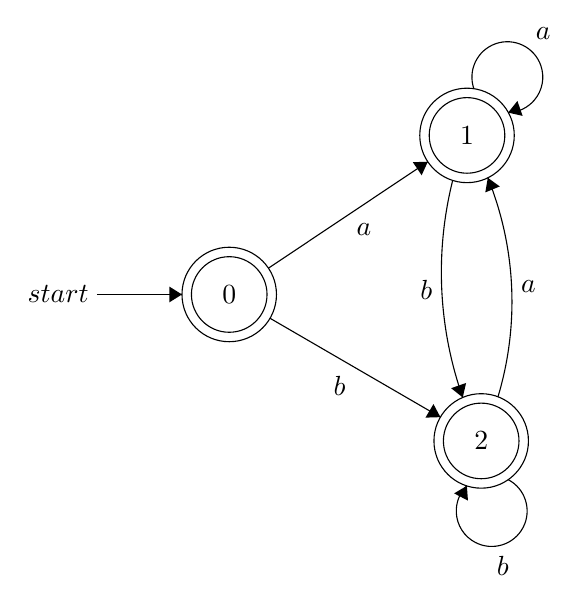
\begin{tikzpicture}[scale=0.2]
        \tikzstyle{every node}+=[inner sep=0pt]
        \draw [black] (16.6,-28.8) circle (3);
        \draw (16.6,-28.8) node {$0$};
        \draw [black] (16.6,-28.8) circle (2.4);
        \draw [black] (31.7,-18.7) circle (3);
        \draw (31.7,-18.7) node {$1$};
        \draw [black] (31.7,-18.7) circle (2.4);
        \draw [black] (32.6,-38.1) circle (3);
        \draw (32.6,-38.1) node {$2$};
        \draw [black] (32.6,-38.1) circle (2.4);
        \draw [black] (19.09,-27.13) -- (29.21,-20.37);
        \fill [black] (29.21,-20.37) -- (28.26,-20.4) -- (28.82,-21.23);
        \draw (25.15,-24.25) node [below] {$a$};
        \draw [black] (19.19,-30.31) -- (30.01,-36.59);
        \fill [black] (30.01,-36.59) -- (29.57,-35.76) -- (29.06,-36.62);
        \draw (23.6,-33.95) node [below] {$b$};
        \draw [black] (32.138,-15.744) arc (199.30485:-88.69515:2.25);
        \draw (36.54,-12.65) node [above] {$a$};
        \fill [black] (34.31,-17.25) -- (35.23,-17.46) -- (34.9,-16.51);
        \draw [black] (31.43,-35.34) arc (-160.61096:-194.07674:23.962);
        \fill [black] (31.43,-35.34) -- (31.64,-34.42) -- (30.69,-34.75);
        \draw (29.53,-28.51) node [left] {$b$};
        \draw [black] (34.305,-40.554) arc (62.53077:-225.46923:2.25);
        \draw (33.97,-45.37) node [below] {$b$};
        \fill [black] (31.69,-40.95) -- (30.88,-41.43) -- (31.76,-41.89);
        \draw [black] (33.021,-21.391) arc (22.04894:-16.73664:20.965);
        \fill [black] (33.02,-21.39) -- (32.86,-22.32) -- (33.78,-21.94);
        \draw (35.1,-28.27) node [right] {$a$};
        \draw [black] (8.2,-28.8) -- (13.6,-28.8);
        \draw (7.7,-28.8) node [left] {$start$};
        \fill [black] (13.6,-28.8) -- (12.8,-28.3) -- (12.8,-29.3);
        \end{tikzpicture}
        \end{center}

        
        $ababbab$

        $0 \to 1 \to 2 \to 1 \to 2 \to 2 \to 1 \to 2 
        $

        \newpage
    \item[c)] \(((\varepsilon|a)b^*)^*\)
    
    $\ec{0} = \{0,1,2,3,4,6,7,9,10\} = S_0 \\
    \ecc{\mv{S_0}{a}} = \ec{5} = \{1,2,3,4,5,6,7,9,10\} = S_1 \\
    \ecc{\mv{S_0}{b}} = \ec{8} = \{1,2,3,4,6,7,8,9,10\} = S_2 \\
    \ecc{\mv{S_1}{a}} = \ec{5} = S_1 \\
    \ecc{\mv{S_1}{b}} = \ec{8} = S_2 \\
    \ecc{\mv{S_2}{a}} = \ec{5} = S_1 \\
    \ecc{\mv{S_2}{b}} = \ec{8} = S_2 \\
    $

    \begin{center}
        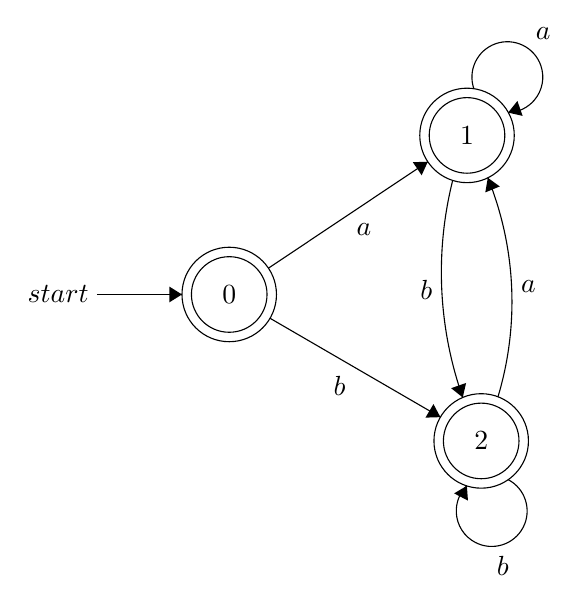
\begin{tikzpicture}[scale=0.2]
        \tikzstyle{every node}+=[inner sep=0pt]
        \draw [black] (16.6,-28.8) circle (3);
        \draw (16.6,-28.8) node {$0$};
        \draw [black] (16.6,-28.8) circle (2.4);
        \draw [black] (31.7,-18.7) circle (3);
        \draw (31.7,-18.7) node {$1$};
        \draw [black] (31.7,-18.7) circle (2.4);
        \draw [black] (32.6,-38.1) circle (3);
        \draw (32.6,-38.1) node {$2$};
        \draw [black] (32.6,-38.1) circle (2.4);
        \draw [black] (19.09,-27.13) -- (29.21,-20.37);
        \fill [black] (29.21,-20.37) -- (28.26,-20.4) -- (28.82,-21.23);
        \draw (25.15,-24.25) node [below] {$a$};
        \draw [black] (19.19,-30.31) -- (30.01,-36.59);
        \fill [black] (30.01,-36.59) -- (29.57,-35.76) -- (29.06,-36.62);
        \draw (23.6,-33.95) node [below] {$b$};
        \draw [black] (32.138,-15.744) arc (199.30485:-88.69515:2.25);
        \draw (36.54,-12.65) node [above] {$a$};
        \fill [black] (34.31,-17.25) -- (35.23,-17.46) -- (34.9,-16.51);
        \draw [black] (31.43,-35.34) arc (-160.61096:-194.07674:23.962);
        \fill [black] (31.43,-35.34) -- (31.64,-34.42) -- (30.69,-34.75);
        \draw (29.53,-28.51) node [left] {$b$};
        \draw [black] (34.305,-40.554) arc (62.53077:-225.46923:2.25);
        \draw (33.97,-45.37) node [below] {$b$};
        \fill [black] (31.69,-40.95) -- (30.88,-41.43) -- (31.76,-41.89);
        \draw [black] (33.021,-21.391) arc (22.04894:-16.73664:20.965);
        \fill [black] (33.02,-21.39) -- (32.86,-22.32) -- (33.78,-21.94);
        \draw (35.1,-28.27) node [right] {$a$};
        \draw [black] (8.2,-28.8) -- (13.6,-28.8);
        \draw (7.7,-28.8) node [left] {$start$};
        \fill [black] (13.6,-28.8) -- (12.8,-28.3) -- (12.8,-29.3);
        \end{tikzpicture}
        \end{center}

        
        $ababbab$

        $0 \to 1 \to 2 \to 1 \to 2 \to 2 \to 1 \to 2 
        $

        \newpage
    
    \item[d)] \((a|b)^* abb (a|b)^*\)
    
    $
    \ec{0} = \{0,1,2,4,7\} = S_0 \\
    \ecc{\mv{S_0}{a}} = \ec{3,8} = \{1,2,3,4,6,7,8\} = S_1 \\
    \ecc{\mv{S_0}{b}} = \ec{5} = \{1,2,4,5,6,7\} = S_2 \\
    \ecc{\mv{S_1}{a}} = \ec{3,8} = S_1 \\
    \ecc{\mv{S_1}{b}} = \ec{5,9} = \{1,2,4,5,6,7,9\} = S_3 \\
    \ecc{\mv{S_2}{a}} = \ec{3,8} = S_1 \\
    \ecc{\mv{S_2}{b}} = \ec{5} = S_2 \\
    \ecc{\mv{S_3}{a}} = \ec{3,8} = S_1 \\
    \ecc{\mv{S_3}{b}} = \ec{5,10} = \{1,2,4,5,6,7,9,10,11,12,14,17\} = S_4 \\
    \ecc{\mv{S_4}{a}} = \ec{3,8,13} = \{1,2,3,4,6,7,8,9,11,12,13,14,16,17\} = S_5 \\
    \ecc{\mv{S_4}{b}} = \ec{5,15} = \{1,2,4,5,6,7,11,12,14,15,16,17\} = S_6 \\
    \ecc{\mv{S_5}{a}} = \ec{3,8,13} = S_5 \\
    \ecc{\mv{S_5}{b}} = \ec{5,9,15} = \{1,2,4,5,6,7,9,11,12,14,15,16,17\} = S_7 \\
    \ecc{\mv{S_6}{a}} = \ec{3,8,13} = S_5 \\
    \ecc{\mv{S_6}{b}} = \ec{5,15} = S_6 \\
    \ecc{\mv{S_7}{a}} = \ec{3,8,13} = S_5 \\
    \ecc{\mv{S_7}{b}} = \ec{5,10,15} = \{1,2,4,5,6,7,10,11,12,14,15,16,17\} = S_8 \\
    \ecc{\mv{S_8}{a}} = \ec{3,8,13} = S_5 \\
    \ecc{\mv{S_8}{b}} = \ec{5,15} = S_6 \\
    $

    \begin{center}
        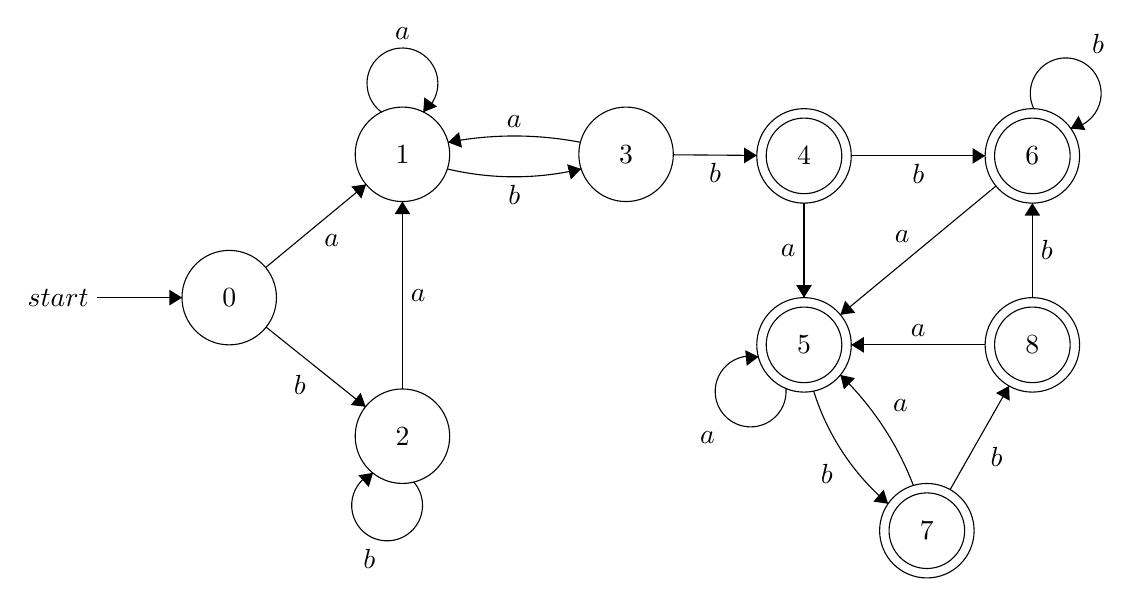
\begin{tikzpicture}[scale=0.2]
        \tikzstyle{every node}+=[inner sep=0pt]
        \draw [black] (16.6,-28.8) circle (3);
        \draw (16.6,-28.8) node {$0$};
        \draw [black] (27.6,-19.7) circle (3);
        \draw (27.6,-19.7) node {$1$};
        \draw [black] (27.6,-37.6) circle (3);
        \draw (27.6,-37.6) node {$2$};
        \draw [black] (41.8,-19.7) circle (3);
        \draw (41.8,-19.7) node {$3$};
        \draw [black] (53.1,-19.8) circle (3);
        \draw (53.1,-19.8) node {$4$};
        \draw [black] (53.1,-19.8) circle (2.4);
        \draw [black] (53.1,-31.8) circle (3);
        \draw (53.1,-31.8) node {$5$};
        \draw [black] (53.1,-31.8) circle (2.4);
        \draw [black] (67.6,-19.8) circle (3);
        \draw (67.6,-19.8) node {$6$};
        \draw [black] (67.6,-19.8) circle (2.4);
        \draw [black] (60.9,-43.6) circle (3);
        \draw (60.9,-43.6) node {$7$};
        \draw [black] (60.9,-43.6) circle (2.4);
        \draw [black] (67.6,-31.8) circle (3);
        \draw (67.6,-31.8) node {$8$};
        \draw [black] (67.6,-31.8) circle (2.4);
        \draw [black] (8.2,-28.8) -- (13.6,-28.8);
        \draw (7.7,-28.8) node [left] {$start$};
        \fill [black] (13.6,-28.8) -- (12.8,-28.3) -- (12.8,-29.3);
        \draw [black] (18.91,-26.89) -- (25.29,-21.61);
        \fill [black] (25.29,-21.61) -- (24.35,-21.74) -- (24.99,-22.51);
        \draw (23.11,-24.74) node [below] {$a$};
        \draw [black] (18.94,-30.67) -- (25.26,-35.73);
        \fill [black] (25.26,-35.73) -- (24.95,-34.84) -- (24.32,-35.62);
        \draw (21.09,-33.69) node [below] {$b$};
        \draw [black] (26.277,-17.02) arc (234:-54:2.25);
        \draw (27.6,-12.45) node [above] {$a$};
        \fill [black] (28.92,-17.02) -- (29.8,-16.67) -- (28.99,-16.08);
        \draw [black] (38.951,-20.629) arc (-76.623:-103.377:18.374);
        \fill [black] (38.95,-20.63) -- (38.06,-20.33) -- (38.29,-21.3);
        \draw (34.7,-21.63) node [below] {$b$};
        \draw [black] (27.6,-34.6) -- (27.6,-22.7);
        \fill [black] (27.6,-22.7) -- (27.1,-23.5) -- (28.1,-23.5);
        \draw (28.1,-28.65) node [right] {$a$};
        \draw [black] (28.31,-40.503) arc (41.47119:-246.52881:2.25);
        \draw (25.5,-44.77) node [below] {$b$};
        \fill [black] (25.73,-39.93) -- (24.8,-40.08) -- (25.46,-40.83);
        \draw [black] (30.499,-18.936) arc (100.90145:79.09855:22.215);
        \fill [black] (30.5,-18.94) -- (31.38,-19.28) -- (31.19,-18.29);
        \draw (34.7,-18.03) node [above] {$a$};
        \draw [black] (44.8,-19.73) -- (50.1,-19.77);
        \fill [black] (50.1,-19.77) -- (49.3,-19.27) -- (49.3,-20.27);
        \draw (47.45,-20.26) node [below] {$b$};
        \draw [black] (53.1,-22.8) -- (53.1,-28.8);
        \fill [black] (53.1,-28.8) -- (53.6,-28) -- (52.6,-28);
        \draw (52.6,-25.8) node [left] {$a$};
        \draw [black] (56.1,-19.8) -- (64.6,-19.8);
        \fill [black] (64.6,-19.8) -- (63.8,-19.3) -- (63.8,-20.3);
        \draw (60.35,-20.3) node [below] {$b$};
        \draw [black] (51.95,-34.558) arc (5.09237:-282.90763:2.25);
        \draw (47.47,-37.69) node [left] {$a$};
        \fill [black] (50.21,-32.56) -- (49.37,-32.14) -- (49.46,-33.13);
        \draw [black] (58.442,-41.888) arc (-130.41307:-162.65617:15.447);
        \fill [black] (58.44,-41.89) -- (58.16,-40.99) -- (57.51,-41.75);
        \draw (54.96,-39.97) node [left] {$b$};
        \draw [black] (65.29,-21.71) -- (55.41,-29.89);
        \fill [black] (55.41,-29.89) -- (56.35,-29.76) -- (55.71,-28.99);
        \draw (59.34,-25.31) node [above] {$a$};
        \draw [black] (67.694,-16.813) arc (205.92751:-82.07249:2.25);
        \draw (71.77,-13.34) node [above] {$b$};
        \fill [black] (70.03,-18.06) -- (70.97,-18.16) -- (70.53,-17.26);
        \draw [black] (55.407,-33.713) arc (45.92788:21.00288:19.483);
        \fill [black] (55.41,-33.71) -- (55.63,-34.63) -- (56.33,-33.91);
        \draw (58.72,-35.64) node [right] {$a$};
        \draw [black] (62.38,-40.99) -- (66.12,-34.41);
        \fill [black] (66.12,-34.41) -- (65.29,-34.86) -- (66.16,-35.35);
        \draw (64.91,-38.92) node [right] {$b$};
        \draw [black] (64.6,-31.8) -- (56.1,-31.8);
        \fill [black] (56.1,-31.8) -- (56.9,-32.3) -- (56.9,-31.3);
        \draw (60.35,-31.3) node [above] {$a$};
        \draw [black] (67.6,-28.8) -- (67.6,-22.8);
        \fill [black] (67.6,-22.8) -- (67.1,-23.6) -- (68.1,-23.6);
        \draw (68.1,-25.8) node [right] {$b$};
        \end{tikzpicture}
        \end{center}

        $ababbab$

        $0 \to 1 \to 3 \to 1 \to 3 \to 4 \to 5 \to 7
        $
\end{enumerate}

\end{document}